\documentclass{beamer}

\usefonttheme{professionalfonts} % using non standard fonts for beamer
\usefonttheme{serif} % default family is serif

\usepackage{hyperref}
%\usepackage{minted}
\usepackage{animate}
\usepackage{graphicx}
\def\Put(#1,#2)#3{\leavevmode\makebox(0,0){\put(#1,#2){#3}}}
\usepackage{color}
\usepackage{tikz}
\usepackage{amssymb}
\usepackage{enumerate}


\newcommand\blfootnote[1]{%

  \begingroup

  \renewcommand\thefootnote{}\footnote{#1}%

  \addtocounter{footnote}{-1}%

  \endgroup

}

\makeatletter

%%%%%%%%%%%%%%%%%%%%%%%%%%%%%% Textclass specific LaTeX commands.

 % this default might be overridden by plain title style

 \newcommand\makebeamertitle{\frame{\maketitle}}%

 % (ERT) argument for the TOC

 \AtBeginDocument{%

   \let\origtableofcontents=\tableofcontents

   \def\tableofcontents{\@ifnextchar[{\origtableofcontents}{\gobbletableofcontents}}

   \def\gobbletableofcontents#1{\origtableofcontents}

 }

%%%%%%%%%%%%%%%%%%%%%%%%%%%%%% User specified LaTeX commands.

\usetheme{Malmoe}

% or ...

\useoutertheme{infolines}

\addtobeamertemplate{headline}{}{\vskip2pt}

\setbeamercovered{transparent}

% or whatever (possibly just delete it)

\makeatother

\begin{document}
\title[PFLOCK report]{PFLOCK Report}
\author[AC]{Andres Calderon}
\institute[Fall'19]{University of California, Riverside}
\makebeamertitle
\newif\iflattersubsect

\AtBeginSection[] {
    \begin{frame}<beamer>
    \frametitle{Outline} 
    \tableofcontents[currentsection]  
    \end{frame}
    \lattersubsectfalse
}

\AtBeginSubsection[] {
    \begin{frame}<beamer>
    \frametitle{Outline} 
    \tableofcontents[currentsubsection]  
    \end{frame}
}

\begin{frame}{Working on ICPE - Range Join}
    \begin{itemize}
        \item The Range Join procedure from ICPE has been implemented.
        \item Algoritms GridAllocate and GridQuery are done and integrated with the previous code.
        \item I have tested the results to find maximal disks with our implementation.  Outputs are identical.
        \item I am re-running the experiments with LA\_10K and LA\_25K for consistency.
    \end{itemize}
\end{frame}

\begin{frame}{Working on Brinkhoff dataset (duplicates records)}
    \begin{itemize}
        \item Keeping 9.5M distinct records aside.
        \item `Fixing' the remaining 12.5M records. For each duplicate record: 
        \begin{itemize}
            \item Create a new Id, move location 1m north-east, keep same time instant.
            \item The slight movement still can generate new duplicates but they were very few.  They were removed accordingly.
        \end{itemize}
        \item The results has 39870 trajectories and 22M points (no duplicates).
    \end{itemize}
\end{frame}

\begin{frame}{What is next?}
    \begin{itemize}
        \item Run experiments with Brinkhoff dataset.
        \item Explore the pattern enumeration strategy proposed on Chen et al. Indeed, I already have worked on the ID-based partitioning technique.
        \item I also would like to explore the use of Spark Streaming to manages trajectories online and be able to use window operations. For example: ...
    \end{itemize}
\end{frame}

\begin{frame}{Window operations}
    \centering
    \begin{figure}
        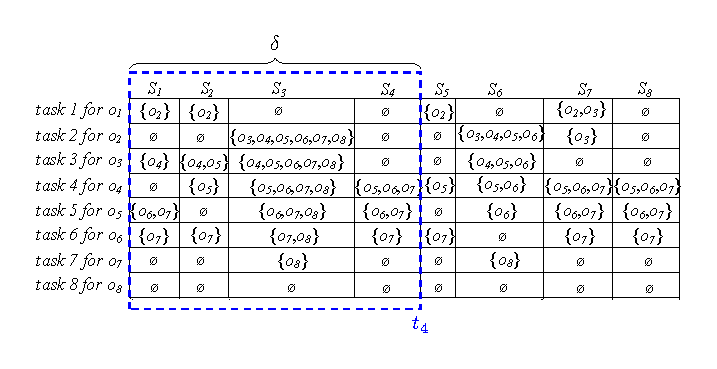
\includegraphics[width=.9\textwidth]{figures/Window01}
    \end{figure}    
\end{frame}
\begin{frame}{Window operations}
    \centering
    \begin{figure}
        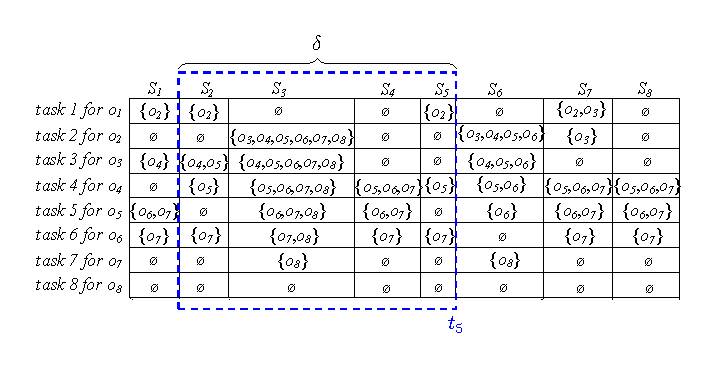
\includegraphics[width=.9\textwidth]{figures/Window02}
    \end{figure}    
\end{frame}
\begin{frame}{Window operations}
    \centering
    \begin{figure}
        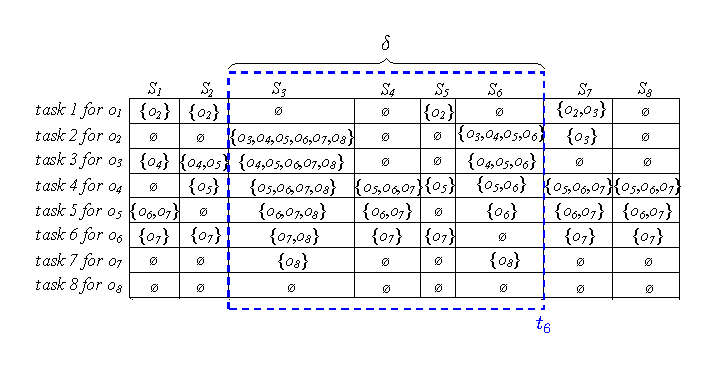
\includegraphics[width=.9\textwidth]{figures/Window03}
    \end{figure}    
\end{frame}
\begin{frame}{Window operations}
    \centering
    \begin{figure}
        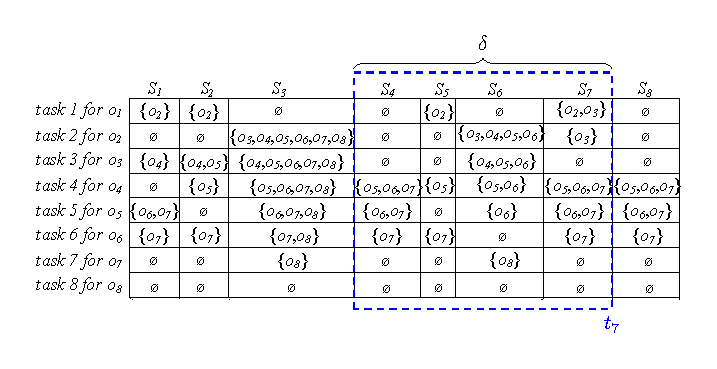
\includegraphics[width=.9\textwidth]{figures/Window04}
    \end{figure}    
\end{frame}
\begin{frame}{Window operations}
    \centering
    \begin{figure}
        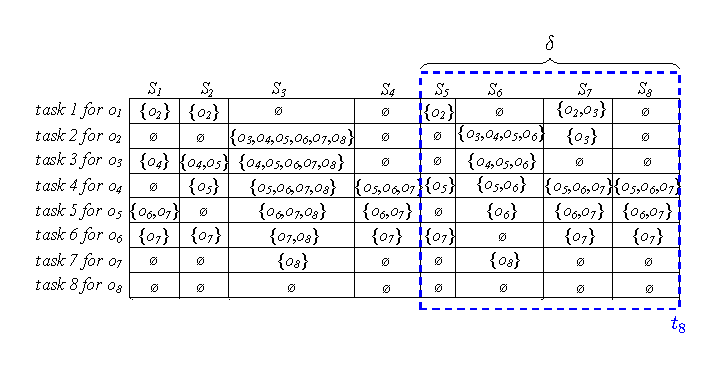
\includegraphics[width=.9\textwidth]{figures/Window05}
    \end{figure}    
\end{frame}


\end{document}
